\section{Planificación del Proyecto}
\label{sec:planificacion}

%La planificación del proyecto se formula a partir del problema identificado y de los requisitos funcionales, no funcionales y ambientales definidos previamente. En esta etapa, el propósito de la planificación es establecer una ruta de trabajo que permita avanzar desde la caracterización de los documentos y del entorno institucional hasta la validación de una solución técnicamente viable.
%La planificación se organiza mediante un objetivo general, objetivos específicos, actividades e hitos. El objetivo general expresa el resultado global esperado, mientras que los objetivos específicos describen los resultados parciales necesarios para alcanzarlo. Cada objetivo específico se asocia con actividades y con un hito verificable que permite comprobar su cumplimiento.

\subsection{Objetivo General}
\label{subsec:objetivo_general}

Desarrollar y validar una solución de transcripción y análisis de documentos históricos digitalizados, basada en herramientas de código abierto y ejecutable en la infraestructura computacional disponible, capaz de recuperar con fidelidad el contenido textual y estructural y de generar información procesable que apoye la homogeneización, indexación y búsqueda documental en DocuDigital.

\subsection{Objetivos Específicos}
\label{subsec:objetivos_especificos}

\begin{enumerate}
    \item[\textbf{OE-01}] Caracterizar los documentos digitalizados considerados por el proyecto, identificando sus categorías, estructuras, condiciones de digitalización, niveles de degradación y elementos de información relevantes, mediante la conformación de un conjunto documental representativo.

    \item[\textbf{OE-02}] Definir un procedimiento reproducible para evaluar alternativas de procesamiento documental, estableciendo documentos de referencia, configuraciones experimentales, métricas de fidelidad y mecanismos para registrar tiempos de ejecución y consumo de recursos.

    \item[\textbf{OE-03}] Evaluar comparativamente alternativas de código abierto para la transcripción y el análisis documental bajo condiciones equivalentes, con el propósito de identificar configuraciones compatibles con las restricciones de infraestructura institucional.

    \item[\textbf{OE-04}] Implementar un prototipo funcional que permita procesar documentos digitalizados, recuperar su contenido textual y estructural y generar representaciones procesables, metadatos y descripciones de contenido.

    \item[\textbf{OE-05}] Validar el prototipo mediante documentos representativos y dentro del entorno computacional disponible, evaluando conjuntamente la fidelidad de los resultados, el tiempo de procesamiento, el consumo de recursos, la estabilidad y la reproducibilidad de la ejecución.
\end{enumerate}


\newcommand{\responsable}{\shortstack[c]{Cristóbal Díaz\\Vilches}}

\subsection{Hitos y Actividades}
\label{subsec:hitos_actividades}


\begingroup
\scriptsize
\renewcommand{\arraystretch}{1.15}
\setlength{\tabcolsep}{1.7pt}
\setlength{\LTleft}{0pt}
\setlength{\LTright}{0pt}
\setlength{\emergencystretch}{2em}
\sloppy

\begin{longtable}{
    >{\centering\arraybackslash}p{1.45cm}
    >{\RaggedRight\arraybackslash}p{6.0cm}
    >{\centering\arraybackslash}p{1.9cm}
    >{\centering\arraybackslash}p{1.65cm}
    >{\centering\arraybackslash}p{1.65cm}
    >{\centering\arraybackslash}p{0.95cm}
}
\caption{Actividades, tareas, resultados de producción e hitos del proyecto.}
\label{tab:hitos_actividades}\\

\toprule
\textbf{\shortstack{Act, \\ ...}} &
\textbf{Descripción resumida} &
\textbf{Responsable} &
\textbf{\shortstack{Fecha\\inicio}} &
\textbf{\shortstack{Fecha\\entrega}} &
\textbf{\shortstack{\% de\\logro}} \\
\midrule
\endfirsthead

\multicolumn{6}{c}{\tablename\ \thetable{} -- continuación} \\
\toprule
\textbf{\shortstack{Act, \\ ...}} &
\textbf{Descripción resumida} &
\textbf{Responsable} &
\textbf{\shortstack{Fecha\\inicio}} &
\textbf{\shortstack{Fecha\\entrega}} &
\textbf{\shortstack{\% de\\logro}} \\
\midrule
\endhead

\midrule
\multicolumn{6}{r}{Continúa en la página siguiente.} \\
\endfoot

\bottomrule
\endlastfoot

\addlinespace[3pt]
\multicolumn{6}{l}{\textbf{OE1 --- Caracterizar el dominio documental y sus restricciones}} \\
\midrule

\textbf{A1.1} &
\textbf{Contextualización institucional y formulación del problema.} &
\responsable &
01/06/2026 &
05/06/2026 &
\textbf{100\%} \\


\addlinespace[2pt]
\textbf{A1.2} &
\textbf{Caracterización del problema de transcripción y comprensión documental.} &
\responsable &
01/06/2026 &
05/06/2026 &
\textbf{100\%} \\


\addlinespace[2pt]
\textbf{A1.3} &
\textbf{Caracterización de restricciones ambientales y definición de requisitos.} &
\responsable &
01/06/2026 &
29/07/2026 &
\textbf{100\%} \\


\addlinespace[2pt]
\textbf{RP1} &
\textbf{Caracterización documental y requisitos del sistema.} &
\responsable &
01/06/2026 &
29/07/2026 &
\textbf{100\%} \\

\textbf{H1.1} &
\textbf{Problema, alcance y requisitos definidos.} &
\responsable &
29/07/2026 &
29/07/2026 &
\textbf{100\%} \\

\midrule
\addlinespace[3pt]
\multicolumn{6}{l}{\textbf{OE2 --- Definir una metodología reproducible de evaluación}} \\
\midrule

\textbf{A2.1} &
\textbf{Definición de referencias verificadas y normalización.} &
\responsable &
22/06/2026 &
03/07/2026 &
\textbf{100\%} \\

\addlinespace[2pt]
\textbf{A2.2} &
\textbf{Selección e implementación de métricas de evaluación.} &
\responsable &
23/06/2026 &
03/07/2026 &
\textbf{100\%} \\

\addlinespace[2pt]
\textbf{A2.3} &
\textbf{Diseño del experimento, captura de recursos y trazabilidad.} &
\responsable &
10/06/2026 &
03/07/2026 &
\textbf{100\%} \\


\addlinespace[2pt]
\textbf{A2.4} &
\textbf{Diseño e implementación del dashboard de resultados.} &
\responsable &
02/07/2026 &
29/07/2026 &
\textbf{100\%} \\

\addlinespace[2pt]
\textbf{RP2} &
\textbf{Protocolo de evaluación y diseño del benchmark.} &
\responsable &
10/06/2026 &
29/07/2026 &
\textbf{100\%} \\

\textbf{H2.1} &
\textbf{Metodología de evaluación disponible.} &
\responsable &
03/07/2026 &
03/07/2026 &
\textbf{100\%} \\

\textbf{H2.2} &
\textbf{Documentación de los diseños y métricas.} &
\responsable &
29/07/2026 &
29/07/2026 &
\textbf{100\%} \\

\midrule
\addlinespace[3pt]
\multicolumn{6}{l}{\textbf{OE3 --- Evaluar alternativas de procesamiento documental de código abierto}} \\
\midrule

\textbf{A3.1} &
\textbf{Investigación y preselección de modelos.} &
\responsable &
01/06/2026 &
19/06/2026 &
\textbf{100\%} \\

\addlinespace[2pt]
\textbf{A3.2} &
\textbf{Preparación de modelos, cuantizaciones y perfiles.} &
\responsable &
08/06/2026 &
26/06/2026 &
\textbf{100\%} \\

\addlinespace[2pt]
\textbf{A3.3} &
\textbf{Ejecución del benchmark comparativo.} &
\responsable &
10/06/2026 &
03/07/2026 &
\textbf{100\%} \\

\addlinespace[2pt]
\textbf{A3.4} &
\textbf{Análisis comparativo y selección.} &
\responsable &
17/06/2026 &
03/07/2026 &
\textbf{100\%} \\

\addlinespace[2pt]
\textbf{RP3} &
\textbf{Evaluación comparativa de modelos y configuraciones.} &
\responsable &
01/06/2026 &
03/07/2026 &
\textbf{100\%} \\

\textbf{H3.1} &
\textbf{Herramienta de visualización y comparación de resultados.} &
\responsable &
03/07/2026 &
03/07/2026 &
\textbf{100\%} \\

\textbf{H3.2} &
\textbf{Alternativa de procesamiento seleccionada.} &
\responsable &
03/07/2026 &
03/07/2026 &
\textbf{100\%} \\

\textbf{H3.3} &
\textbf{Benchmark integrado y reproducible.} &
\responsable &
26/06/2026 &
26/06/2026 &
\textbf{100\%} \\

\midrule
\addlinespace[3pt]
\multicolumn{6}{l}{\textbf{OE4 --- Implementar un prototipo de transcripción y análisis documental}} \\
\midrule

\textbf{A4.1} &
\textbf{Diseño de arquitectura, módulos e interfaces.} &
\responsable &
06/07/2026 &
29/07/2026 &
\textbf{100\%} \\


\addlinespace[2pt]
\textbf{A4.2} &
\textbf{Implementación del flujo de preprocesamiento e inferencia.} &
\responsable &
08/07/2026 &
20/07/2026 &
\textbf{100\%} \\

\addlinespace[2pt]
\textbf{A4.3} &
\textbf{Generación de salida estructurada, metadatos y descripciones.} &
\responsable &
20/07/2026 &
02/10/2026 &
\textbf{50\%} \\

\addlinespace[2pt]
\textbf{A4.4} &
\textbf{Integración local y manejo robusto de ejecuciones.} &
\responsable &
13/07/2026 &
21/08/2026 &
\textbf{80\%} \\

\addlinespace[2pt]
\textbf{RP4} &
\textbf{Prototipo funcional de procesamiento documental.} &
\responsable &
08/07/2026 &
23/10/2026 &
\textbf{82.5\%} \\

\textbf{H4.1} &
\textbf{Procesamiento documental de extremo a extremo.} &
\responsable &
20/07/2026 &
20/07/2026 &
\textbf{100\%} \\

\textbf{H4.2} &
\textbf{Servicio OCR, CLI y API operativos.} &
\responsable &
23/07/2026 &
23/07/2026 &
\textbf{100\%} \\

\midrule
\addlinespace[3pt]
\multicolumn{6}{l}{\textbf{OE5 --- Validar y documentar la solución en el entorno institucional}} \\
\midrule

\textbf{A5.1} &
\textbf{Preparación del conjunto final de validación.} &
\responsable &
22/06/2026 &
06/11/2026 &
\textbf{50\%} \\

\addlinespace[2pt]
\textbf{A5.2} &
\textbf{Validación de fidelidad y eficiencia.} &
\responsable &
15/06/2026 &
20/11/2026 &
\textbf{66.7\%} \\

\addlinespace[2pt]
\textbf{A5.3} &
\textbf{Pruebas de estabilidad y procesamiento por lotes.} &
\responsable &
20/07/2026 &
27/11/2026 &
\textbf{60\%} \\

\addlinespace[2pt]
\textbf{A5.4} &
\textbf{Documentación técnica, académica y recomendaciones.} &
\responsable &
21/07/2026 &
11/12/2026 &
\textbf{75\%} \\

\addlinespace[2pt]
\textbf{RP5} &
\textbf{Solución validada y documentación técnica.} &
\responsable &
15/06/2026 &
11/12/2026 &
\textbf{62.9\%} \\

\textbf{H5.1} &
\textbf{Solución validada y documentada.} &
\responsable &
11/12/2026 &
11/12/2026 &
\textbf{0\%} \\

\end{longtable}

\endgroup



\subsection{Carta Gantt}

\begin{figure}[H]
    \centering
    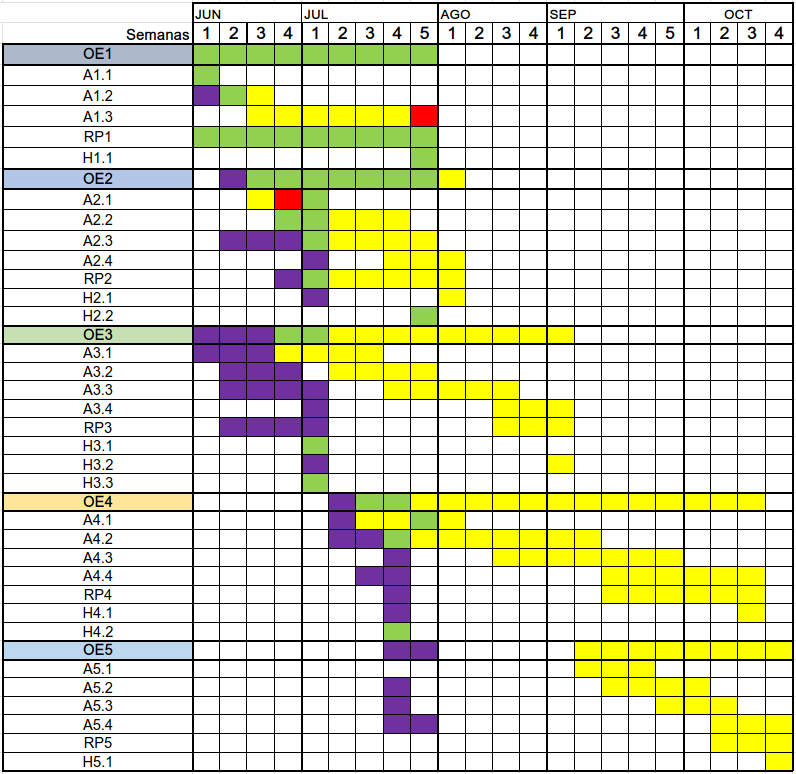
\includegraphics[width=1.0\linewidth]{images/Gantt.png}
    \caption{Carta Gantt}
    \label{fig:gantt}
\end{figure}

\begin{figure}[H]
    \centering
    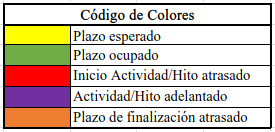
\includegraphics[width=0.4\linewidth]{images/coloresGantt.png}
    \caption{Codigo de colores de Carta Gantt}
    \label{fig:colorGantt}
\end{figure}
